\documentclass[a4paper,twoside,onecolumn]{article}
\usepackage[english]{babel}
\usepackage{verbatim}
\usepackage{colortbl}
\usepackage{pifont}
\usepackage{fancyhdr}
\usepackage{fancyvrb}
\usepackage{fancybox}
\usepackage{dblfloatfix}
\usepackage{amsmath}
\usepackage{tabularx}
\usepackage{setspace}
\usepackage{amssymb}
\usepackage{amsbsy}
\usepackage{alltt}
\usepackage[Bjornstrup]{fncychap}
\usepackage{graphicx}
\usepackage[centering,includeheadfoot,margin=2cm]{geometry}
\usepackage{color}
\usepackage[colorlinks=true,urlcolor=blueback,linktoc=page,linkcolor=black]{hyperref}
\usepackage{makeidx}

\definecolor{blueback}{RGB}{10,31,98}
\definecolor{grayback}{RGB}{54,54,54}

%\renewcommand{\topfraction}{0.1}	% max fraction of floats at top
%\renewcommand{\bottomfraction}{0.1}	% max fraction of floats at bottom
%\setcounter{topnumber}{1}
%\setcounter{bottomnumber}{1}
%\setcounter{totalnumber}{1}     % 2 may work better
%\setcounter{dbltopnumber}{1}    % for 2-column pages
%\renewcommand{\dbltopfraction}{0}	% fit big float above 2-col. text
%\renewcommand{\textfraction}{1}	% allow minimal text w. figs
%\renewcommand{\floatpagefraction}{1}	% require fuller float pages
%\renewcommand{\dblfloatpagefraction}{0}	% require fuller float pages

\newcommand{\etexttt}[1]{\textit{#1}}

\definecolor{MyGray}{rgb}{0.95,0.95,0.95}
\newenvironment{colframe}{% 
  \begin{Sbox} 
    \begin{minipage}{.8\columnwidth} 
}{% 

  \end{minipage} 
  \end{Sbox} 
  \begin{center} 
    \fcolorbox{black}{MyGray}{\TheSbox} 
  \end{center} 
} 

\setlength\fboxrule{1pt}
\addtolength{\headheight}{2.5pt}
\fancyhead[LE]{\rightmark}
\fancyhead[RO]{\leftmark}
\fancyhead[RE]{ModelCC User Manual}
\fancyhead[LO]{ModelCC User Manual}
\lfoot[\thepage]{}
\rfoot[]{\thepage}
\cfoot[]{}
\renewcommand{\headrulewidth}{0.4pt}
\renewcommand{\footrulewidth}{0.4pt}
\usepackage{fancyvrb}

\newcommand{\pb}{\newpage}
\newcommand{\empt}{\pb \thispagestyle{empty} \rule[0mm]{0mm}{0mm} \pb}
\newcommand{\an}[1]{\emph{#1}} %texttt

\begin{document}


\begin{titlepage}

\begin{center}

\rule{0cm}{3cm}

\includegraphics[width=1.00\textwidth]{logo.eps}\\[-1.5cm]
\hfill {\color{blueback} \bf v\input{version} (\input{releasedate}\unskip)} \rule{0.17cm}{0cm}\\[2cm]

\textsc{\color{blueback} \bf \Huge User Manual}\\[0.2cm]
\rule{0cm}{1cm}

\end{center}

\rule{0cm}{9cm}
{\color{blueback} \bf\LARGE\unskip The ModelCC Development Team\hfill {\large \href{http://www.modelcc.org/}{www.modelcc.org}}}
\begin{itemize}
\item[\color{blueback}\scalebox{0.9}{\textbullet}] {\color{blueback} \bf\large Luis Quesada (\href{mailto:lquesada@modelcc.org}{lquesada@modelcc.org})}
\item[\color{blueback}\scalebox{0.9}{\textbullet}] {\color{blueback} \bf\large Fernando Berzal (\href{mailto:berzal@modelcc.org}{berzal@modelcc.org})}
\item[\color{blueback}\scalebox{0.9}{\textbullet}] {\color{blueback} \bf\large Francisco J. Cortijo (\href{mailto:cb@modelcc.org}{cb@modelcc.org})}
\item[\color{blueback}\scalebox{0.9}{\textbullet}] {\color{blueback} \bf\large Juan-Carlos Cubero (\href{mailto:jc.cubero@modelcc.org}{jc.cubero@modelcc.org})}
\end{itemize}

\end{titlepage}


%\empt
%\empt
%\empt
%\empt
%\empt

%\pagestyle{empty}

%\begin{center}

%\rule{0cm}{3cm}
%
\includegraphics[width=1.00\textwidth]{logog.eps}\\[-1.5cm]
%\hfill {\color{grayback} \bf v\input{version} (\input{releasedate}\unskip)} \rule{0.17cm}{0cm}\\[2cm]
%
%\textsc{\color{grayback} \bf \Huge User Manual}\\[0.2cm]
%\rule{0cm}{1cm}
%
%\end{center}

%\rule{0cm}{9cm}

%\empt
%\empt
%\empt

\pagestyle{empty}

\tableofcontents

\cleardoublepage

\pagestyle{fancy}

\newpage
\section{Introduction} 

ModelCC is a model-based parser generator that decouples language specification from language processing.

The idea behind model-based language specification is that, starting from a single abstract syntax model (ASM) representing the core concepts in
a language, language designers would later develop one or several concrete syntax models (CSMs). These concrete syntax models would suit the
specific needs of the desired textual or graphical representation. The ASM-CSM mapping could be performed, for instance, by annotating the
abstract syntax model with the constraints needed to transform the elements in the abstract syntax into their concrete representation.


Section \ref{sec:modelspec} comments on ModelCC building blocks.

Section \ref{sec:modelcons} describes the model constraints supported by ModelCC, which declaratively define the features of the formal language defined by the model.

Section \ref{sec:asmcsm} presents an example of use of the ModelCC Domain Specific Language for ASM-CSM mapping.

Section \ref{sec:predefinedtypes} defines ModelCC predefined types.

Section \ref{sec:gettingstarted} explains how to use ModelCC.

Section \ref{sec:examples} exposes examples of languages specified using ModelCC.

Section \ref{sec:testing} presents an example of model testing using ModelCC testing framework.

\section{Model Specification} \label{sec:modelspec}

Any class implementing the \emph{IModel} interface is considered a language element.

The specification of a language in ModelCC starts with the definition of basic language elements, which might be viewed as the tokens in the model-driven specification of a language.
Basic language elements can be modeled as simple classes in an object-oriented programming language annotated with pattern constraints, as described in Section \ref{subsec:patterns}.
The ASM-CSM mapping of those basic elements will establish their correspondence to the tokens that appear in the concrete syntax of the language whose ASM we design in ModelCC.

The metadata annotation \emph{@Setup} can be used to specify the method, if any, that has to be run to initialize the language element instances.

Then, ModelCC provides the necessary mechanisms to combine those basic elements into more complex language constructs, which correspond to the use of concatenation, selection, and repetition in the syntax-driven specification of languages.

In the following subsections, we describe the mechanisms provided by ModelCC to implement the three main constructs that let us specify complete abstract syntax models on top of basic
language elements.

\subsection{Concatenation}

Concatenation is the most basic construct we can use to combine sets of language elements into more complex language elements.

In ModelCC, concatenation is achieved by object composition. The resulting language element is the composite element and its members are the language elements the composite element collates.

The following code shows an example of object composition, in which an \emph{AssignmentStatement} is composed of an \emph{Identifier} and an \emph{Expression}:

\begin{colframe}
\begin{alltt}
import org.modelcc.*;

public class AssignmentStatement implements{\emph IModel} \{

  {\bf Identifier id;}

  {\bf Expression exp;}

\}
\end{alltt}
\end{colframe}

\subsection{Selection}

Selection allows the specification of alternative elements in language constructs.

In ModelCC, selection is achieved by subtyping. Specifying inheritance relationships among language elements in an object-oriented context
corresponds to defining `is-a' relationships. The language element we wish to establish alternatives for is the superelement, whereas the different alternatives are
represented as subelements.

The following code shows an example of selection, in which an \emph{Expression} can be either an \emph{UnaryExpression}, a \emph{BinaryExpression}, or a \emph{ParenthesizedExpression}:

\begin{colframe}
\begin{alltt}
import org.modelcc.*;

public class Expression implements{\emph IModel} \{

\}
\end{alltt}
\end{colframe}

\begin{colframe}
\begin{alltt}
import org.modelcc.*;

public class UnaryExpression{\bf extends Expression} implements{\emph IModel} \{

\}
\end{alltt}
\end{colframe}

\begin{colframe}
\begin{alltt}
import org.modelcc.*;

public class BinaryExpression{\bf extends Expression} implements{\emph IModel} \{

\}
\end{alltt}
\end{colframe}

\begin{colframe}
\begin{alltt}
import org.modelcc.*;

public class ParenthesizedExpression{\bf extends Expression}
                                                       implements{\emph IModel} \{

\}
\end{alltt}
\end{colframe}

\subsection{Repetition}

Repetition allows the specification of a language element that appears several times in a given language construct.

In ModelCC, repetition is also achieved through object composition, just by allowing different multiplicities in the associations that connect
composite elements to their constituent elements, that is, by declaring container members such as arrays, Lists/ArrayLists, or Sets/HashSets.
The cardinality constraints described in Section \ref{subsec:cardinality} can be used to annotate ModelCC models in order to establish specific multiplicities for repeatable language elements.

The following five pieces of code show examples of repetition, in which an \emph{OutputStatement} can contain an array, a List, an ArrayList, a Set, or an HashSet of \emph{Expressions}.

\begin{colframe}
\begin{alltt}
import org.modelcc.*;

public class OutputStatement extends Statement implements{\emph IModel} \{

  {\bf\unskip Expression[] exp;}

\}
\end{alltt}
\end{colframe}

\begin{colframe}
\begin{alltt}
import org.modelcc.*;

public class OutputStatement extends Statement implements{\emph IModel} \{

  {\bf\unskip List\(<\)Expression\(>\) exp;}

\}
\end{alltt}
\end{colframe}

\begin{colframe}
\begin{alltt}
import org.modelcc.*;

public class OutputStatement extends Statement implements{\emph IModel} \{

  {\bf\unskip ArrayList\(<\)Expression\(>\) exp;}

\}
\end{alltt}
\end{colframe}

\begin{colframe}
\begin{alltt}
import org.modelcc.*;

public class OutputStatement extends Statement implements{\emph IModel} \{

  {\bf\unskip Set\(<\)Expression\(>\) exp;}

\}
\end{alltt}
\end{colframe}

\begin{colframe}
\begin{alltt}
import org.modelcc.*;

public class OutputStatement extends Statement implements{\emph IModel} \{

  {\bf\unskip HashSet\(<\)Expression\(>\) exp;}

\}
\end{alltt}
\end{colframe}


\section{Model Constraints} \label{sec:modelcons}

Once we have examined the mechanisms that let us create abstract syntax models in ModelCC, we now proceed to describe how constraints can be imposed on such models in order to establish the desired ASM-CSM mapping.
As soon as that ASM-CSM mapping is established, ModelCC is able to generate the suitable parser for the concrete syntax defined by the CSM.

ModelCC allows the definition of constraints using metadata annotations or a domain-specific language.

In ModelCC, which supports language composition without being scannerless, a first set of constraints is used for pattern specification, a necessary feature for defining the lexical elements of the concrete syntax model, i.e. its tokens (Subsection \ref{subsec:patterns}).

A second set of constraints is employed for defining delimiters in the concrete syntax model, whose use is common for eliminating language ambiguities or just as syntactic sugar in many languages (Subsection \ref{subsec:delimiters}).

A third set of ModelCC constraints lets us impose cardinalities on language elements, which control element repeatability and optionality (Subsection \ref{subsec:cardinality}).

A fourth set of constraints lets us impose evaluation order on language elements, which are employed to declaratively resolve further ambiguities in the concrete syntax of a textual language by establishing associativity, precedence, and composition policies, the latter employed, for example, for resolving the ambiguities that cause the typical shift-reduce conflicts in LR parsers (Subsection \ref{subsec:evalorder}).

A fifth set of constraints lets us specify the element constituent order in composite elements. (Subsection \ref{subsec:comporder}).

A sixth set of constraints lets us specify referenceable language elements and references to them (Subsection \ref{subsec:references}).

Custom constraints let us provide specific lexical, syntactic, and semantic constraints that take into consideration context information (Subsection \ref{subsec:custom}).

Finally, probability constraints let us specify probabilities for disambiguation (Subsection \ref{subsec:probability}).

\subsection{Pattern Specification Constraints} \label{subsec:patterns}

Pattern specification constraints allow the specification of the lexical elements in a concrete syntax model, i.e. the different token types defined for the concrete syntax of a textual language.
It should be noted that, once a language element is annotated with pattern specification constraints, it cannot be a composite element since, as a lexical element, it cannot be composed of other elements.

The above constraint, which forces lexical elements to be basic language elements in a ModelCC ASM, does not reduce the flexibility of ModelCC for language composition.
Language composition, typically achieved by scannerless parser generators, can also be achieved if the scanner supports lexical ambiguities.
When lexical ambiguities are allowed, the same string or even overlapping strings might correspond to several tokens, which will later be processed by the parser consuming the output of the scanner supporting lexical ambiguities.

\subsubsection{The @Pattern annotation}

\begin{figure}[tb!]
\begin{minipage}{\linewidth}
\centering

\includegraphics[scale=1]{identifier.eps}
\caption{Pattern specification example: Regular expression.} \label{fig:identifier}
\end{minipage}

\vspace{1mm}
\begin{minipage}{\linewidth}

\begin{center} \begin{minipage}{7.1cm} \vspace{4mm}
\begin{verbatim}

[a-zA-Z][_a-zA-Z0-9]*  return Identifier;
\end{verbatim}
\vspace{-6mm} \end{minipage} \end{center}

\caption{Implementation of Figure \ref{fig:identifier} in lex.}
\label{fig:identifierg}

\end{minipage}

\vspace{3mm}
\begin{minipage}{\linewidth}
\centering

\includegraphics[scale=1]{javadoc.eps}
\caption{Pattern specification example: Custom pattern matching.} \label{fig:javadoc}
\end{minipage}

\end{figure}

The \an{@Pattern} annotation allows the specification of the pattern that will be used to match a basic language element in the input string.
Two mutually exclusive mechanisms are provided for pattern specification in ModelCC: regular expressions and user-defined pattern matching classes.
Regular expressions can be specified in ModelCC to build standard lexers, whereas custom pattern matching classes allow the language designer to use any custom-defined matching element to recognize basic language elements in the input string.
The custom pattern matching class can be anything, since it works as a black box for ModelCC.
It might even be a complete ModelCC-generated parser, which could be used for the specification of modular languages, a coarse form of language composition (e.g. think of the JavaScript scripts and CSS stylesheets within the
HTML in a web page).

When used with regular expressions, the \an{@Pattern} annotation includes an argument representing the regular expression.
This regular expression, specified as the \emph{regExp} field of the annotation, corresponds to the traditional token type definition in lex-like scanners.

When used with custom pattern matching classes, the \an{@Pattern} annotation is used to specify the name of the class implementing the matching algorithm and its argument string.
If this pattern specification mechanism is used, ModelCC will need to resort to a scanning algorithm that supports pattern matcher classes.

For example, the \an{@Pattern} annotation in Figure \ref{fig:identifier} defines the typical \emph{Identifier} token in programming languages, which can be specified by the following regular expression: \emph{[a-zA-Z][\_a-zA-Z0-9]*}.
This specification corresponds to the lex token definition shown in Figure \ref{fig:identifierg}.

The example in Figure \ref{fig:javadoc} illustrates the use of custom pattern matching classes in ModelCC.
In this case, the \an{@Pattern} annotation refers to the \emph{JavaDocRecognizer} class, which will be responsible for recognizing \emph{JavaDoc} comments as basic language elements in the shown ASM.
Arguments can also be specified when using the \emph{matcher} field of the \an{@Pattern} annotation with the help of its optional \emph{args} field (\emph{``simple''} in Figure \ref{fig:javadoc}).

As mentioned above, the ModelCC use of custom pattern matching algorithms for defining basic language elements has no counterpart in traditional lexer generators, hence an equivalent lex-like definition cannot be provided.

\subsubsection{The @Value annotation}

The \an{@Value} annotation can be used in ModelCC to indicate the location where the recognized token value will be stored in the abstract syntax graph, so that value can be used once the input string has been parsed.

\begin{figure}[tb!]
\begin{minipage}{\linewidth}
\centering

\includegraphics[scale=1]{integerliteral.eps}
\caption{Value field specification example: Integer literals.}
 \label{fig:integerliteral}
\end{minipage}


\begin{minipage}{\linewidth}
\begin{center} \begin{minipage}{5cm} \vspace{4mm}
\begin{verbatim}

[0-9]+ {
  yylval.value = atoi(yytext);
  return INTEGERLITERAL;
}
\end{verbatim}
\vspace{-6mm} \end{minipage} \end{center}
\caption{Implementation of Figure \ref{fig:integerliteral} using lex \& yacc.} \label{fig:integerliteralg}
\end{minipage}
\vspace{3mm}

\begin{minipage}{\linewidth}
\centering

\includegraphics[scale=1]{stringliteral.eps}
\caption{Value field specification example: Double-quoted string literals.} \label{fig:stringliteral}
\end{minipage}


\begin{minipage}{\linewidth}
\begin{center} \begin{minipage}{5.2cm} \vspace{4mm}
\begin{verbatim}

\"[^\"]*\" {
  int size,csize;
  size = strlen(yytext);
  csize = sizeof(char)*(size+1);
  yylval.pval = malloc(csize);
  strncpy(yylval.pval,yytext,size);
  return STRINGLITERAL;
}
\end{verbatim}
\vspace{-6mm} \end{minipage} \end{center}
\caption{Implementation of Figure \ref{fig:stringliteral} using lex \& yacc.} \label{fig:stringliteralg}
\end{minipage}

\end{figure}

Associated to a field of the class defining a basic language element, that field will contain the value obtained from the input string that matches the token type pattern specification.

When a numeric or boolean field is annotated with the \an{@Value} annotation, it is not necessary to specify the corresponding \an{@Pattern} annotation for recognizing the numeric or boolean tokens. When the \an{@Value}-annotated field is not numeric nor boolean (e.g. a string, a single character, or any non-primitive data type), the use of the \an{@Pattern} annotation is mandatory.

Elements from the ASM that contain a \an{@Value}-annotated numeric or boolean field are transformed into their corresponding token type lex-like definitions, even when no \an{@Pattern} annotation is present.
ModelCC will always perform the proper assignment of the recognized token to the \an{@Value}-annotated field.

For example, the model in Figure \ref{fig:integerliteral} defines an \emph{IntegerLiteral} language element that recognizes long integer literals.
The proper regular expression for such literals will be employed and, whenever an integer literal is found in the input string, its integer value will be stored in the \an{@Value}-annotated \emph{value} field of the \emph{IntegerLiteral} class.
If we had used lex \& yacc, we would have had to type the lexical definition and semantic action shown in Figure \ref{fig:identifierg}.

As another example, Figure \ref{fig:stringliteral} shows how the \an{@Value} annotation would be used in conjunction with the \an{@Pattern} annotation to define string literals surrounded by double quotes.
A \emph{StringLiteral} will be recognized whenever a pair of double quotes encloses a string not containing a double quote, a constraint that can be specified by the following regular expression: \emph{$\backslash$``[$\mathbin{\char`\^}\backslash$``]*$\backslash$``}.
The lex \& yacc implementation of this string literal token type definition would be slightly more complex than the previous example, as shown in Figure \ref{fig:stringliteralg}.

\subsection{Delimiter Constraints} \label{subsec:delimiters}

Delimiter constraints allow the specification of language element delimiters in a concrete syntax model. Delimiters include prefixes, suffixes, and separators.
Such kinds of delimiters are often used to eliminate language ambiguities and facilitate parsing, but they can appear just as syntactic sugar to make languages more readable.

Usually, reserved words in programming languages act just as delimiters.
As such, they will not appear in the language abstract syntax model.
They will be specified as metadata annotations in the ASM-CSM mapping corresponding to the concrete syntax of the language.

It should be noted that delimiters should always be specified as constraints on the ASM-CSM mapping rather than language elements in the ASM, since they do not provide any relevant information from the perspective of the abstract syntax model, even though they might be necessary to define unambiguous textual languages.

\subsubsection{The @Prefix annotation}

The \an{@Prefix} annotation allows the specification of prefixes for language elements and specific constituents in composite language elements.

The \emph{value} field of the \an{@Prefix} annotation is used to specify the list of regular expressions that define the prefixes that precede the corresponding language element (or a specific constituent element within a composite element) in the concrete syntax of a textual CSM.

When converting the ASM into a textual CSM, ModelCC will include the specified prefixes in every production where the annotated element appears in the textual CSM grammar, just before the appearance of the annotated element.
When the annotation is associated to a constituent element within a composite language element, the sequence of prefixes will be included only in the productions that correspond to the composite language element, preceding the annotated constituent element within their right-hand side.

It should be noted that, when the annotated element is repeatable, the sequence of prefixes appear only once, preceding the first instance of the annotated element.
Prefixes will also be included in the CSM even when no elements appear in a repetition language construct (e.g. as when the opening parenthesis appears before an empty list of arguments in a parameterless C-like function call), but not when the repetition language construct is optional and is not present.

For example, the model in Figure \ref{fig:programmain} specifies that the textual representation of a \emph{Program} will always be preceded by a ``main'' keyword prefix.
The grammar defining the textual CSM for this simple example is  \etexttt{$<$ProgramMain$>$ ::= ``main'' $<$Statement$>$}.

\begin{figure}[tb!]
\centering
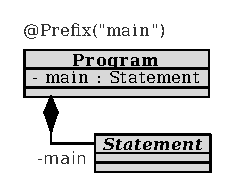
\includegraphics[scale=1]{programmain.eps}
\caption{\an{@Prefix} annotation example.} \label{fig:programmain}
\end{figure}



\subsubsection{The @Suffix annotation}

The \an{@Suffix} annotation allows the specification of suffixes for language elements and specific constituents in composite language elements.

The \emph{value} field of the \an{@Suffix} annotation is used to specify the list of regular expressions that define the suffixes that follow the corresponding language element (or a specific constituent element within a composite element) in the concrete syntax of a textual CSM.

When converting the ASM into a textual CSM, ModelCC will include the specified suffixes in every production where the annotated element appears in the textual CSM grammar, just after the appearance of the annotated element.
When the annotation is associated to a constituent element within a composite language element, the sequence of suffixes will be included only in the productions that correspond to the composite language element, following the annotated constituent element within their right-hand side.

It should be noted that, when the annotated element is repeatable, the sequence of suffixes appear only once, just after the last element in the sequence of repetitions.
Suffixes will also be included in the CSM even when no elements appear in a repetition language construct (e.g. as when the closing parenthesis appears at the end of an empty list of arguments in a parameterless C-like function call), but not when the repetition language construct is optional and is not present.

For example, the model in Figure \ref{fig:inputstatement} specifies that the textual representation of an \emph{InputStatement} is preceded by an ``input'' keyword prefix and followed by a semicolon (``;'') as its suffix.
It also contains a sequence of \emph{Identifier}s delimited by opening and closing parentheses: ``('' as the prefix of the \emph{ids} constituent of the \emph{InputStatement} composite and ``)'' as its suffix.
The grammar defined by the ASM-CSM mapping specified by the annotations in Figure \ref{fig:inputstatement} is \etexttt{$<$InputStatement$>$ ::= ``input'' ``('' $<$IdentifierList$>$ ``)'' ``';''; $<$IdentifierList$>$ ::= $<$Identifier$>$ $<$IdentifierList$>$ $|$ $<$Identifier$>$}.

\begin{figure}[tb!]
\centering
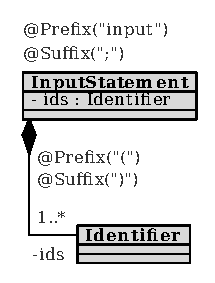
\includegraphics[scale=1]{inputstatement.eps}
\caption{\an{@Suffix} annotation example.} \label{fig:inputstatement}
\end{figure}

\subsubsection{The @Separator annotation}

The \an{@Separator} annotation allows the specification of separators between consecutive instances of elements within a repetition.
Separators can be defined in ModelCC by annotating a language element in the ASM or just its appearance within a particular repetition construct.
In the first case, a default separator is established for the language element: the specified separator will be used for separating consecutive instances of the annotated language element whenever a sequence of such language elements appears in a textual CSM.
In the second case, an \emph{ad hoc} separator is defined: the specified separator will be used only when consecutive instances of the language element appear within the context of the annotated repetition construct.

The \emph{ad hoc} definition of separators with the \an{@Separator} annotation within repetition constructs can be used to override or disable the default sequence of separators associated to the repeatable element in a repetition construct.

Therefore, default separators are specified for language elements by the \an{@Separator} annotation.
When converting the ASM into a textual CSM, ModelCC will include the sequence of regular expressions defining those default separators in every recursive production rule generated from a repetition where the annotated element is repeatable.
When the \an{@Separator} annotation accompanies a repeatable element within a particular repetition construct, i.e. the \emph{ad hoc} case, separators will only appear in the recursive production rule derived from that particular repetition construct, but not in other constructs where the constituent element might also be repeatable.

As an example of defining a default separator, Figure \ref{fig:identifier2} illustrates how a comma (``,'') can be used as the default separator for \emph{Identifier}s.
Whenever a list of \emph{Identifier}s is needed within the language, a comma will separate consecutive identifiers.
In the example, since a \emph{VariableDeclaration} contains a \emph{Type} and a set of \emph{Identifier}s, they will be separated by ``,'' in the textual CSM derived from the language ASM.
The grammar of the resulting CSM will include the following productions: \etexttt{$<$VariableDeclaration$>$ ::= $<$Type$>$ $<$IdentifierList$>$ ``;''} and \etexttt{$<$IdentifierList$>$ ::= $<$Identifier$>$ ``,'' $<$IdentifierList$>$ $|$ $<$Identifier$>$}.

\begin{figure}[tb!]
\centering
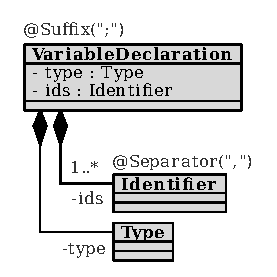
\includegraphics[scale=1]{identifier2.eps}
\caption{Default \an{@Separator} example.} \label{fig:identifier2}
\end{figure}

As an example illustrating the use of \emph{ad hoc} separators, consider the model in Figure \ref{fig:inputstatement2}.
Here, \emph{Identifier}s are also separated by commas, but only within \emph{InputStatement}s, i.e. ``,'' is the \emph{ad hoc} separator for identifiers within input statements, but lists of identifiers might employ different separators elsewhere.
The grammar associated to the textual CSM derived from Figure \ref{fig:inputstatement2} would include the following productions: \etexttt{$<$InputStatement$>$ ::= ``input'' ``('' $<$InputStatementIdentifierList$>$ ``)'' ``;''} and \etexttt{$<$InputStatementIdentifierList$>$ ::= $<$Identifier$>$ ``,'' $<$InputStatementIdentifierList$>$ $|$ $<$Identifier$>$}.

\begin{figure}[tb!]
\centering
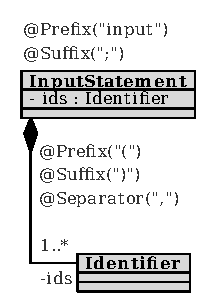
\includegraphics[scale=1]{inputstatement2.eps}
\caption{\emph{Ad hoc} \an{@Separator} example.} \label{fig:inputstatement2}
\end{figure}

\subsection{Cardinality Constraints} \label{subsec:cardinality}

Cardinality constraints let us impose cardinalities on composite language elements, which control element repeatability and optionality.

\subsubsection{The @Optional annotation}

The \an{@Optional} annotation allows the specification of optional elements in textual CSMs.

Optional elements naturally appear in language specifications and optionality could always be modeled by means of selection constructs.
However, the declarative specification of the optionality constraints is necessary to avoid unnecessary duplication in the language model.

When one of the constituent elements within a composite language element is optional, the textual representation of the composite element might include the optional element along with its corresponding delimiters, or not.
In the latter case, the missing element delimiters are not included in the textual representation either, even though a prefix and a suffix might have been defined for the missing constituent element.

If we performed a naive transformation of a composite language into a set of CFG production rules and the composite element includes $i$ optional elements, $2^i$ production rules would result with the composite element in their left-hand side and all the possible combinations of optional elements in their right-hand side.
A more reasonable transformation employs just $2i$ ancillary production rules that represent whether if each optional element is to be matched or not.

For example, the model in Figure \ref{fig:conditional2} shows that a \emph{ConditionalStatement} contains an \emph{Expression}, the \emph{Statement} that will be run when the \emph{Expression} evaluates to true, and, optionally, the \emph{Statement} that will be run when the \emph{Expression} evaluates to false.
The grammar resulting from the model transformation into a textual CSM will include the following two productions: \etexttt{$<$ConditionalStatement$>$ ::= ``if'' $<$Expression$>$ $<$Statement$>$ $<$OptionalElse$>$} and \etexttt{$<$OptionalElse$>$ ::= ``else'' $<$Statement$>$ $|$ $\epsilon$}.

\begin{figure}[tb!]
\centering
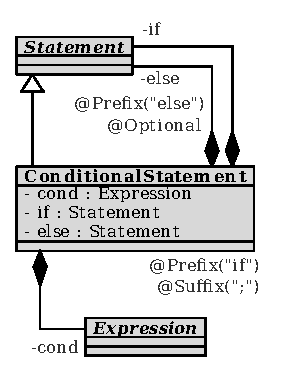
\includegraphics[scale=1]{conditional2.eps}
\caption{\an{@Optional} element example: if-then-else statement.} \label{fig:conditional2}
\end{figure}

\subsubsection{The @Multiplicity annotation}

The \an{@Multiplicity} annotation, depicted as minimum and maximum multiplicity constraint in standard UML notation, allows the specification of the lower and upper bound for the multiplicity of repeatable language elements within repetition constructs.
By default, the lower bound is $0$ and the upper bound is infinite.

It should be noted that, when the minimum multiplicity is $0$, no elements might appear in a particular instance of the repetition.
However, delimiters would still be represented in the textual CSM unless the \an{@Optional} annotation were explicitly employed.

ModelCC generates semantic predicates that check if specific bounds are met for a list of elements, in which case the generated parser would not recognize the list of elements as such, since it does not satisfy the cardinality constraint imposed by the multiplicity annotation.

Other parser generators would require the explicit generation of a grammar representing the minimum and maximum cardinality constraint, i.e. when an element must appear at least $i$ times within a repetition, two production rules would be necessary: \etexttt{$<$MinIElements$>$ ::= $<$Element$>$... i times... $<$Element$>$ $<$ElementList$>$} and \etexttt{$<$ElementList$>$ ::= $<$Element$>$ $<$ElementList$>$ $|$ $\epsilon$}.

For example, the model in Figure \ref{fig:arguments} indicates that a \emph{Program} might have from $0$ to $2$ \emph{Parameter}s.
Here, the multiplicity annotation is inferred from the multiplicity of the UML association.
The grammar corresponding to the textual CSM derived from Figure \ref{fig:arguments} would include the following production rules: \etexttt{$<$Program$>$ ::= $<$OptionalParameterList$>$; $<$OptionalParameterList$>$ ::= $<$ParameterList$>$ $|$ $\epsilon$; and $<$ParameterList$>$ ::= $<$Parameter$>$ $<$ParameterList$>$ $|$ $<$Parameter$>$}, where the last production would be accompanied by a semantic predicate that would check whether the maximum multiplicity constraint holds.
If such feature were not available in our parsing algorithm generator, this last production would have to be replaced by a much more explicit (and potentially verbose) set of equivalent productions incorporating the maximum multiplicity constraint: \etexttt{$<$ParameterList$>$ ::= $<$Parameter$>$ $|$ $<$Parameter$>$ $<$Parameter$>$}.
This approach poses no problems in this simple example, but it might get much more complicated (no problem yet whenever the resulting grammar is automatically generated by a model-driven language specification tool).

\begin{figure}[tb!]
\centering
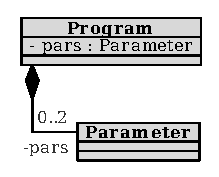
\includegraphics[scale=1]{arguments.eps}
\caption{Maximum multiplicity example.} \label{fig:arguments}
\end{figure}

\subsection{Evaluation Order Constraints} \label{subsec:evalorder}

Evaluation order constraints let us declaratively resolve syntactic ambiguities in the concrete syntax of a textual language by establishing associativity, composition, and precedence constraints for CSMs.

\subsubsection{The @Associativity annotation}

The \an{@Associativity} annotation allows the specification of the operator-like associativity of language elements.
ModelCC supports the following options for specifying associativity constraints:

\begin{itemize}
\item \an{UNDEFINED}, when no associativity is declared (by default), all possibilities are considered.
\item \an{LEFT\_TO\_RIGHT}, for left-associative operations (e.g. subtraction, division, or function application).
\item \an{RIGHT\_TO\_LEFT}, for right-associative elements (e.g. exponentiation and function definition).
\item \an{NON\_ASSOCIATIVE}, for non-associative elements (e.g. cross of three vectors).
\end{itemize}

The specification of associativity constrains help us resolve ambiguities that might appear in recursive compositions (i.e. when using the composite design pattern for modeling the ASM for operations without explicit delimiters), where different interpretations of the input string could be given unless the associativity constraints impose an order on the reductions that can be performed (either left-to-right or right-to-left).

For each production in the CSM grammar where the nonterminal of a language element with associativity constraints is preceded and/or followed by the nonterminal that appears on the left-hand side the production or any of its superclasses in the ASM, ModelCC generates a semantic predicate that enforces that associativity constraint.
The associativity constraint can be implemented by inhibiting the reduction of a production in three situations:

\begin{itemize}
\item Whenever the element that follows a left-to-right associative element was generated by a reduction of the same production.
\item Whenever the element that precedes a right-to-left associative element was generated by a reduction of the same production.
\item Whenever an element that precedes or follows a non-associative element was generated by a reduction of the same production.
\end{itemize}

For example, the model in Figure \ref{fig:operator} establishes that \emph{BinaryOperator}s are left-associative.
The grammar for the resulting textual CSM would include the productions \etexttt{$<$Expression$>$ ::= $<$BinaryExpression$>$} and \etexttt{$<$BinaryExpression$>$ ::= $<$Expression$>$ $<$BinaryOperator$>$ $<$Expression$>$}, where associativity is not explicit.
Left-associativity will be imposed by the corresponding parser semantic predicate.

\begin{figure}[tb!]
\centering
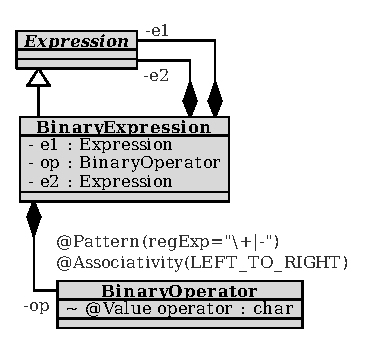
\includegraphics[scale=1]{operator.eps}
\caption{Associativity constraint example.} \label{fig:operator}
\end{figure}

\subsubsection{The @Composition annotation}

\begin{figure}[tb!]
\centering
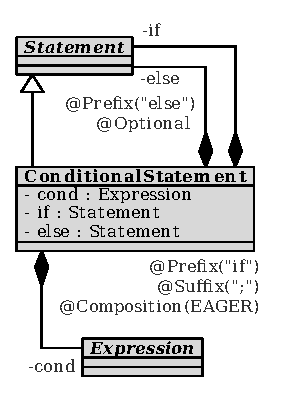
\includegraphics[scale=1]{conditional3.eps}
\caption{Composition constraint example.}
\label{fig:conditional3}
\end{figure}

The \an{@Composition} annotation allows the specification of the suitable order of evaluation of compositions represented in a CSM, a situation that appears whenever the composite design pattern is present in the ASM, no delimiters are employed to eliminate potential ambiguities, and the composite contains several consecutive components of the same type of the composite.
When such composites are nested, different interpretations are possible unless we specify composition constraints in the CSM.
This is the case of the typical shift-reduce conflicts that appear in LR parsers when parsing nested if-then-else statements.

Hence, a specific constraint on element composition must be used to enforce a particular interpretation of such nested compositions in the ASM-CSM mapping.
ModelCC supports the following options for composition constraints:

\begin{itemize}
\item \an{UNDEFINED}, when no composition constraints are defined and potential ambiguities are taken into account.
\item \an{EAGER}, when the matching of constituent elements is performed as soon as possible.
      This corresponds to the typical interpretation of nested if-then-else statements in programming languages, where the else clause is attached to the innermost if statement.
\item \an{LAZY}, when the matching of constituent elements is deferred as much as possible.
      Then, a rightmost derivation is obtained; i.e. when an element might accompany any of two nested language constructs, it is associated to the outermost one.
\item \an{EXPLICIT}, when no composition constraints are defined and any ambiguities should be resolved with the help of delimiters.
\end{itemize}

Composition order constraints are enforced by defining precedences for the productions in the grammar of the resulting textual CSM.
Establishing such precedences is possible in most parsing tools, including all yacc  derivatives and Fence.
When composition is eager, shift operations will precede reduce operations.
In contrast, when composition is lazy, reduce operations will have precedence over shift operations.
Finally, when the composition order must be explicit in the CSM, the use of delimiters will determine whether shift or reduce operations are performed on a case by case basis.

For example, the model in Figure \ref{fig:conditional3} represents typical if-then-else statements.
In this case, the optional else \emph{Statement} of the eager \emph{ConditionalStatement} will always match the innermost if statement when such statements are nested, e.g. in
``if E1 if E2 S1 else S2'', the else clause will correspond to the E2 if statement.
The grammar for the resulting CSM will include the following productions: \etexttt{$<$ConditionalStatement$>$ ::= ``if'' $<$Expression$>$ $<$Statement$>$ ``;'' $|$ ``if'' $<$Expression$>$ $<$Statement$>$ ``else'' $<$Statement$>$ ``;''}.
The parser will enforce the precedence of the second alternative over the first one, so that else clauses are parsed as usual.

\subsubsection{The @Priority annotation}

The \an{@Priority} annotation allows the specification of precedences among language elements for eliminating ambiguities in textual CSMs.

ModelCC implements two mechanisms to specify priority constraints in the ASM-CSM mapping:

\begin{itemize}
\item A relative one, where precedence relationships are established between particular language elements (a \emph{precedes} declaration indicates which language elements have lower priority than the current element).
\item An absolute one, where a numeric priority \emph{value} determines the priority level for each language element (the lower the value, the higher the priority)
\end{itemize}

\begin{figure}[tb!]
\centering
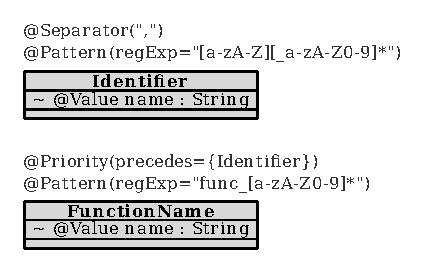
\includegraphics[scale=1]{identifier3.eps}
\caption{Relative priority resolved by the lexical analyzer.} \label{fig:identifier3}
\end{figure}


\begin{figure}[tb!]
\centering
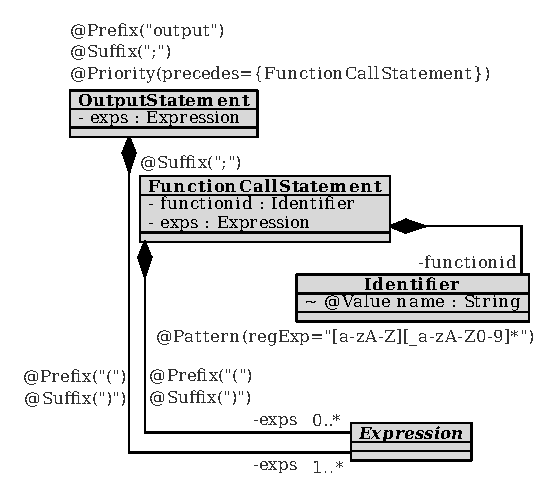
\includegraphics[scale=1]{outputfunction.eps}
\caption{Relative priority resolved by the syntactic analyzer.} \label{fig:outputfunction}
\end{figure}

Unless specified otherwise, all language elements have the same priority.
Precedences established among basic language elements are managed at the lexical analysis level by the corresponding lexer.
Precedences established among non-basic language elements that appear in concatenation, selection, and repetition constructs within the CSM are managed at the syntactic analysis level by the corresponding parser.

For example, the model in Figure \ref{fig:identifier3} establishes a (fictitious) relative priority constraint between function names and identifiers: a \emph{FunctionName} will always precede an \emph{Identifier}.
In case a string like ``func\_power'' is found in the input string, it will be recognized as a \emph{FunctionName}, but not as an \emph{Identifier}.
Since the constraint is defined over basic language elements, the lexical analyzer generated by ModelCC will be responsible for identifying the right element in the input string.

Figure \ref{fig:outputfunction} shows another example.
In this case, the model enforces relative priority constraints between composite language elements that will be resolved by the parser generated by ModelCC.
Here, output statements precede function calls so that a string like ``output(3+5,4+1);'' will be recognized as an \emph{OutputStatement} but not as an \emph{FunctionCallStatement}, even when ``output'' would be a perfectly valid identifier.
The ModelCC lexer, which supports lexical ambiguities, will consider ``output'' as an \emph{Identifier} and also as a delimiter for output statements (i.e. its prefix keyword in the CSM).

\subsection{Composition Order Constraints} \label{subsec:comporder}

The default order of the component elements in a composite element is given by the order in which the composition relationships were specified.
However, composition order constraints let us override the element constituent order in composite elements.

\subsubsection{The @Position Annotation}

\begin{figure}[tb!]
\centering
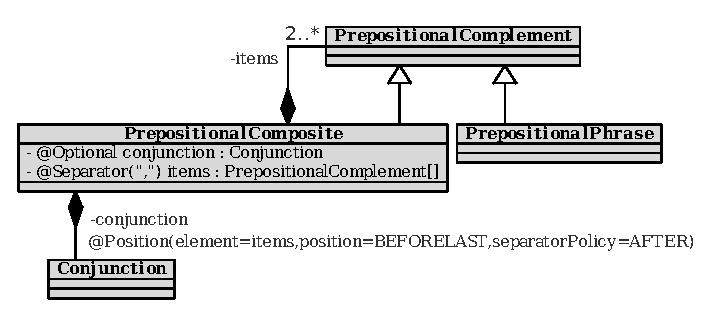
\includegraphics[scale=1]{prepositional.eps}
\caption{Position constraint example.} \label{fig:prepositional}
\end{figure}


The \an{@Position} annotation allows the specification of the position of a component element relative to other component element.
ModelCC supports combinations of the following options for specifying composition order:

\begin{itemize}
\item \an{BEFORE}, when the annotated element appears before the target element.
\item \an{AFTER}, when the annotated element appears after the target element.
\item \an{WITHIN}, when the annotated element appears as an embedded element in a repetition language construct.
\item \an{BEFORELAST}, when the annotated element appears before the last element in a repetition language construct.
\end{itemize}

When the annotated element can appear as part of a repetitive construct (e.g. \an{WITHIN} or \an{BEFORELAST} in an enumeration), ModelCC allows the following separator policies:

\begin{itemize}
\item \an{BEFORE}, when the annotated element appears before the separator.
\item \an{AFTER}, when the annotated element appears after the separator.
\item \an{EXTRA}, when the annotated element appears between separators.
\item \an{REPLACE}, when the annotated element replaces the corresponding separator.
\end{itemize}

The specification of position constraints allow the definition of CSMs in which element constituents are in different order than the composition relationships.
Position constraints also allow embedding an element into a repetitive construct.

The implementation of position constraints in ModelCC consists in generating a set of grammar production that contains all the element orderings that comply with the constraints.
When the target element in a position constraint is a repetitive construct, an ancillary production that includes the embedded element in the corresponding position is produced.

The model in Figure \ref{fig:prepositional} presents an example in which a \emph{PrepositionalComposite} is composed of two or more \emph{PrepositionalComplement}s and an optional conjunction which, in case is present, precedes the last \emph{PrepositionalComplement} in the construct.
The grammar for the resulting textual CSM would include the production \etexttt{$<$PrepositionalComplementList+Conjuntion$>$ ::= $<$PrepositionalComplementList$>$ ``,'' $<$Conjunction$>$ $<$PrepositionalComplement$>$} and, finally, \etexttt{$<$PrepositionalComplementList+Conjuntion$>$ ::= $<$PrepositionalComplementList$>$} due to the optionality of the \emph{Conjunction}.

\subsubsection{The @FreeOrder Annotation}

\begin{figure}[tb!]
\centering
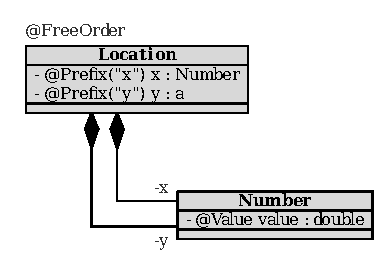
\includegraphics[scale=1]{programfree.eps}
\caption{Free order constraint example.} \label{fig:programfree}
\end{figure}

The \an{@FreeOrder} annotation allows the members of a language element to be shuffled in their textual representation.

When using the \an{@FreeOrder} annotation, ModelCC generates grammar productions for each of the valid orderings of constituent elements in the annotated element.

As an example of the use of the @FreeOrder annotation, the model in Figure \ref{fig:programfree} specifies that a \emph{Location} consists of an ``x'' coordinate and an ``y'' coordinate which may appear in any order.
The grammar defining the textual CSM for this example contains \etexttt{$<$Location$>$ ::= ``x'' $<$Number$>$ ``y'' $<$Number$>$} and \etexttt{$<$Location$>$ ::= ``y'' $<$Number$>$ ``x'' $<$Number$>$}.

\subsection{Reference Constraints} \label{subsec:references}

Reference constraints let us specify referenceable language elements and references to them.

References in ModelCC can be anaphoric, when they are preceded by the corresponding object definition, but also cataphoric, when the references precede the definition, and even recursive, when they appear within the definition they refer to.

\subsubsection{The @ID annotation}

The \an{@ID} annotation allows the specification of the identifier of referenceable language elements.
This annotation is applied to a subset of the members of a language element model.
This subset determines the syntax of references to particular instances of such elements in the concrete syntax of the corresponding language.
That is, any appearance of the same set of values will be interpreted as a reference to the same instance of the referred language element.

It should be noted that the \an{@ID} annotation is incompatible with the \an{@Optional} ModelCC annotation, as null language element identifiers are not allowed, for the same reasons that attributes in a primary key are not nullable in a relational database.
However, the \an{@ID} annotation can be used together with other ModelCC annotations, such as \an{@FreeOrder}, which allows the members of a language element to be shuffled in their textual representation, and \an{@Prefix} and \an{@Suffix}, which add syntactic sugar to the incarnation of the abstract syntax model as a concrete textual language.

The use of references is resolved in our implementation of ModelCC by the introduction of grammar productions that characterize such references and semantic predicates that map them to the corresponding language elements.
The inadvertent definition of two entities of the same class with the same identifier in the same scope results in a runtime warning produced by ModelCC when parsing its input.

In the model in Figure \ref{fig:graphuserref}, the \an{@ID} annotation is employed to identify an \emph{User} by a single number. The grammar for the resulting CSM will contain the traditional \etexttt{$<$User$>$ ::= $<$Number$>$ $<$Name$>$} production with an associated semantic predicate that maps the \emph{Number} identifier of the language element with a particular \emph{User}, and also an additional \etexttt{$<$UserRef$>$ ::= $<$Number$>$} production with an associated semantic predicate that follows the mapping from the \emph{Number} identifier to the particular referenced \emph{User}, if possible.

\begin{figure}[tb!]
\centering
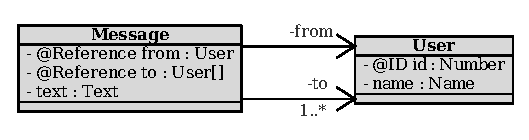
\includegraphics[scale=1]{msg.eps}
\caption{Reference constraint example.}
\label{fig:graphuserref}
\end{figure}

\subsubsection{The @Reference annotation}

The \an{@Reference} annotation allows the specification of references to language elements.
The \an{@Reference} annotation applies to individual members of any language element, provided that the referenced types contain at least one \an{@ID}-annotated member in their language model.

Whenever a language element member is annotated with \emph{@Reference}, the corresponding grammar productions are modified so that they refer to the symbol corresponding to the element reference specification rather than the symbol that corresponds to its full specification.
These productions are then associated to a semantic predicate that resolves the references at the end of the parsing process, in order to support cataphoric and recursive references, apart from the anaphoric references that could be resolved on the fly during the parsing process.

In the example model in Figure \ref{fig:graphuserref}, the \an{@Reference} annotation is employed so that a \emph{Message} contain references to the sender and the recipient \emph{User}s. The grammar for the resulting CSM will contain, apart from the aforementioned \etexttt{$<$UserRef$>$ ::= $<$Number$>$} production and its associated semantic predicate, a \etexttt{$<$Message$>$ ::= $<$UserRef$>$ $<$UserRefList$>$ $<$Text$>$} production, a recursive production of the form \etexttt{$<$UserRefList$>$ ::= $<$UserRef$>$ $<$UserRefList$>$} and a complementary production \etexttt{$<$UserRefList$>$ ::= $<$UserRef$>$}.

\subsubsection{The @Scope annotation}

The \an{@Scope} annotation allows the specification of static reference scopes and applies to language elements.

Dynamic resolution can in general only be determined at run time, therefore dynamic scopes cannot be implemented in the ASM-CSM mapping.

ModelCC supports the following options for static scopes:

\begin{itemize}
\item \an{NESTED}, when the scope nests into the parent scope.
      When resolving references, definitions are looked for by climbing in the scope hierarchy up to the global scope until the identifier is found.
\item \an{LOCAL}, when the scope is local to the instance.
      When resolving references, only definitions inside the language element instance are looked for.
\item \an{GLOBAL}, when the scope is global.
      When resolving references, only definitions inside the global scope are looked for.
\end{itemize}

Whenever a language element member is annotated with \emph{@Scope}, the corresponding grammar productions are modified so that they include scope tags in the mapping of identifiers to definitions. The semantic predicates that correspond to reference resolution only perform the search in the selected scopes.

\begin{figure}[tb!]
\centering
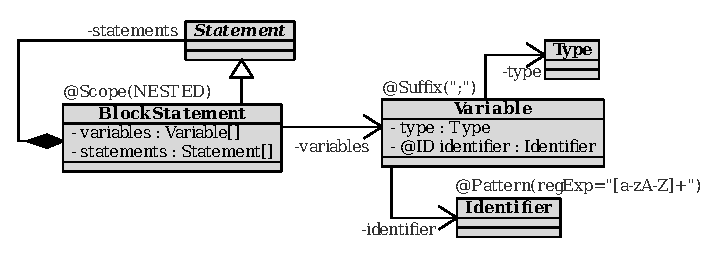
\includegraphics[scale=1]{blockscope.eps}
\caption{Scope constraint example.}
\label{fig:blockscope}
\end{figure}

In the example model in Figure \ref{fig:blockscope}, the \an{@Scope} annotation is used so that each \emph{BlockStatement} defines a new nested scope for variables.

\subsection{Custom constraints with the @Constraint Annotation} \label{subsec:custom}

While ModelCC supports a wide range of constraints, specific situations may require complex lexical, syntactic, or semantic constraints.
ModelCC custom constraints allow the specification of actions that will determine, during the parsing process, whether an instance of a language element is valid or not.

The \an{@Constraint} annotation allows the definition of user-defined methods that are evaluated whenever an instance of the language element is created during the parsing.
The constraining method can take into consideration any of the element members and must return a boolean from its evaluation.
When the return value of the constraining method is ``true'', the element complies with the custom constraints and it is generated.
Contrarily, when the return value of the constraining method is ``false'', the element does not comply with the custom constraints and it is inhibited from generating.

ModelCC directly translates custom constraints into lexer and parser runtime semantic predicates.

The model in Figure \ref{fig:stringliteral2} presents an example in which the \an{@Constraint} annotation is employed so that the \emph{checkEscapedCharacters} user-defined method checks that all escaped characters in a \emph{StringLiteral} are valid (e.g. ``\textbackslash a'' would yield a badly-escaped character error, since the character `a' does not need escaping).

\begin{figure}[tb!]
\centering
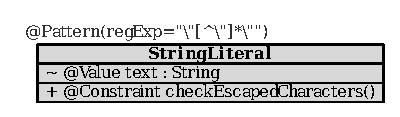
\includegraphics[scale=1]{stringliteral2.eps}
\caption{Custom constraint example.}
\label{fig:stringliteral2}
\end{figure}

\subsection{Probability constraints with the @Probability annotation} \label{subsec:probability}

The \emph{@Probability} annotation allows the specification of probability values for language elements and language element members. Probability values can be specified for syntactic elements of the languages and for lexical components, in which case it should be noted that the lexical analyzer behaves as a part-of-speech tagger in natural language processing.

Such probability values can be specified using ttwo alternatives: a probability value as a real number between $0$ and $1$ or a custom probability evaluator that computes the probability value from the analysis of the language element and its context.

Since ModelCC supports lexical and syntactic ambiguities and the combination of language models, one of the main novelties of ModelCC with respect to existing techniques is that it allows the modular specification of probabilistic languages, that is, it is able to produce parsers from composite language specifications even when some of the language elements overlap or conflict.

ModelCC also supports alternative models for the representation of uncertainty, provided that an evaluation operator for language element instances is provided and an evaluation operator for the application of grammar rules is provided.
Optionally, a casting operator that translates the estimated value in one model into a value valid for a different kind of model allows the specification of modular languages even when different mechanisms for representing natural language ambiguities are employed for different parts of the language model.

\section{ModelCC Domain-Specific Language for ASM-CSM mapping} \label{sec:asmcsm}

The ModelCC DSL for ASM-CSM mapping allows the specification of set of constraints.
By applying such a set of constraint to a model, a new model is obtained.

An example of application of a mapping is:

\begin{colframe}
\begin{verbatim}
import static org.modelcc.csm.CSM;

    Model model = ...
    Model model2 = CSM.apply(model,string/reader);
\end{verbatim}
\end{colframe}

An example of valid input is:

\begin{colframe}
\begin{verbatim}
Element freeorder = true;
Element pattern="[a-z]+";
Element[member] prefix="\\(" suffix="\\)";
\end{verbatim}
\end{colframe}

\section{Predefined types} \label{sec:predefinedtypes}

ModelCC provides several predefined models for common data types.

These models are found in the package org.modelcc.types and are:

\begin{itemize}
\item BooleanModel: A model that recognizes boolean values (``true'' or ``false'').
\item DecimalModel: A model that recognizes signed or unsigned decimal numbers.
\item UnsignedDecimalModel: A model that recognizes unsigned decimal numbers.
\item SignedDecimalModel: A model that recognizes signed decimal numbers.
\item IntegerModel: A model that recognizes signed or unsigned integer numbers.
\item UnsignedIntegerModel: A model that recognizes unsigned integer numbers.
\item SignedIntegerModel: A model that recognizes signed integer numbers.
\item StringModel: A model that recognizes both strings delimited by quotes (with escaped quotes inside) and strings not delimited by quotes.
\item NonQuotedStringModel: A model that recognizes strings not delimited by quotes.
\item QuotedStringodel: A model that recognizes strings delimited by quotes (with escaped quotes inside).
\end{itemize}

\section{Getting Started on ModelCC} \label{sec:gettingstarted}

This section explains how to use ModelCC.

Subsection \ref{sec:install} shows how to set ModelCC up.

Subsection \ref{sec:lang} explains how to implement an example language model.

Subsection \ref{sec:generating} comments on how to generate and use a parser from a language model.

\subsection{Setting up ModelCC} \label{sec:install}

You can get started to ModelCC in a few very easy steps.

\subsubsection{Downloading ModelCC}

Be sure to agree with the ModelCC Shared Software License before downloading ModleCC.

\begin{enumerate}
\item Download the ModelCC binary distribution package (modelcc-[version].zip) from the ModelCC site (www.modelcc.org).
\item Extract it.
\end{enumerate}

\subsubsection{Setting up ModelCC in a NetBeans project}

(If you are not planning on using ModelCC in NetBeans, you may skip this section.)

Whenever you want to use ModelCC in a NetBeans project, you have to add the ModelCC library to it.

\begin{enumerate}
\item Right click your project.
\item Go to {\bf Properties}.
\item Go to the {\bf Libraries} tab.
\item In the {\bf Compile} tab (which is open by default), click the {\bf Add JAR/Folder...} button.
\item Go to the directory where you extracted {\bf modelcc-[version].zip} and select {\bf ModelCC.jar}. Do not select ModelCCExamples.jar, which is a stand-alone application for testing example languages.
\item Accept.
\end{enumerate}

\subsubsection{Setting up ModelCC in an Eclipse project}

(If you are not planning on using ModelCC in Eclipse, you may skip this section.)

Whenever you want to use ModelCC in an Eclipse project, you have to add the ModelCC library to it.

\begin{enumerate}
\item Right click your project.
\item Go to {\bf Properties}.
\item Go to the {\bf Java Build Path} section.
\item In the {\bf Libraries} tab, click the {\bf Add External JARs...} button.
\item Go to the directory where you extracted {\bf modelcc-[version].zip} and select {\bf ModelCC.jar}. Do not select ModelCCExamples.jar, which is a stand-alone application for testing example languages.
\item Accept.
\end{enumerate}

\subsection{Implementing an example language model} \label{sec:lang}

The following class describes a very simple language. The entity {\bf MySimpleLanguage} is a lexical entity that consists of an integer value, which is deducted from the {\bf @Value} annotation that is assigned to an int data type. Any integer number pertains to this language.

\begin{colframe}
\begin{alltt}
import org.modelcc.*;

public class MySimpleLanguage implements IModel {

    @Value
    private int data;    
    
    public int getData() {
        return data;
    }

}
\end{alltt}
\end{colframe}

More complex example languages can be found in the Examples section of the ModelCC site (www.modelcc.org) and in the {\bf ModelCCExamples} library, which is included in the source and binary distribution packages of ModelCC.

\subsection{Generating and using a parser for the example language model} \label{sec:generating}

The parser generation step consists of reading the model of a language and generating a parser from the model.

Subsection \ref{sec:reading} explains how to read the model of a language.
Subsection \ref{sec:genpar} explains how to generate a parser from the language model.
Subsection \ref{sec:usepar} explains how to use the parser.

\subsubsection{Reading the model of a language} \label{sec:reading}

The \emph{Model} class stores language models.

A model can be readed by using a \emph{ModelReader}.

ModelCC currently provides \emph{JavaModelReader}, which is able to produce a model from a set of annotated classes. The following code illustrates the usage of this model reader:

\begin{colframe}
\begin{alltt}
import org.modelcc.io.ModelReader;
import org.modelcc.io.java.JavaModelReader;
import org.modelcc.metamodel.Model;


[...]

//being MySimpleLanguage the main model class.

try \{
  ModelReader jmr = new JavaModelReader(MySimpleLanguage.class);
  Model m = jmr.read();
\} catch (Exception e) \{
  System.out.println(e.getMessage());
\}
\end{alltt}
\end{colframe}

When JavaModelReader is instantiated that way, it provides the \emph{getWarnings()} method, which returns a list of Strings corresponding to the warnings generated during the model reading.

The following code illustrates another way to use this model reader:

\begin{colframe}
\begin{alltt}
import org.modelcc.io.java.JavaModelReader;
import org.modelcc.metamodel.Model;

[...]

//being MySimpleLanguage the main model class.

try \{
  Model m = JavaModelReader.read(MySimpleLanguage.class);
\} catch (Exception e) \{
  System.out.println(e.getMessage());
\}
\end{alltt}
\end{colframe}


\subsubsection{Generating a parser from the language model} \label{sec:genpar}

A \emph{Parser} can be generated from a model.

ModelCC currently provides \emph{ParserFactory}, which is able to produce a Fence parser with a subyacent Lamb lexer from a model and an optional \emph{skip} model which determines the patterns that should be ignored by the lexer (i.e. comments). It should be noted that, in the current implementation, the Lamb lexer ignores any character that does not match a pattern, and the \emph{skip} model can be used to ignore patterns that would be matched as other tokens. The following code illustrates the usage of this parser generator:

\begin{colframe}
\begin{alltt}
import org.modelcc.metamodel.Model;
import org.modelcc.parser.Parser;
import org.modelcc.parser.ParserFactory;

[...]

//being m the model.

try \{
  Parser<MySimpleLanguage> parser = ParserFactory.create(m,ParserFactory.WHITESPACE);
\} catch (Exception e) \{
  System.out.println(e.getMessage());
\}
\end{alltt}
\end{colframe}

The following code illustrates the usage of this parser generator with a \emph{skip} model:

\begin{colframe}
\begin{alltt}
import org.modelcc.metamodel.Model;
import org.modelcc.parser.Parser;
import org.modelcc.parser.ParserFactory;

[...]

//being m the model.
//being skip the skip model.
//being MySimpleLanguage the main model class.

try \{
  Parser<MySimpleLanguage> parser = ParserFactory.create(m,skip);
\} catch (Exception e) \{
  System.out.println(e.getMessage());
\}
\end{alltt}
\end{colframe}

\subsubsection{Using the parser} \label{sec:usepar}

After the parser has been generated, it accepts strings or readers as input and produce instances of the main class. The parser provides several methods that produce different sets of results, considering one or several interpretation (in the case of ambiguities). The following code illustrates the usage of the parser:

\begin{colframe}
\begin{alltt}
import org.modelcc.parser.Parser;

[...]

//being parser a Parser<MySimpleLanguage>.
//being MySimpleLanguage the main model class.
//being input an input String or Reader.

MySimpleLanguage result = parser.parse(input);
\end{alltt}
\end{colframe}

The parser also provide the \emph{parseAll} method, which return a \emph{Collection} of instances of the main class, one for each possible interpretation; and the \emph{parseIterator} method, which return an \emph{Iterator} to the instances of the main class, which allows considering each possible interpretation.

\subsubsection{Full example} \label{sec:fullexample}

The following code reads a model from a set of annotated Java classes, generates a parser, and uses it to generate an object instance from an input string:

\begin{colframe}
\begin{alltt}
import org.modelcc.io.java.JavaModelReader;
import org.modelcc.metamodel.Model;
import org.modelcc.parser.Parser;
import org.modelcc.parser.ParserFactory;

[...]

try \{

  // Read the language model.
  Model m = JavaModelReader.read(Expression.class);

  // Generate a parser from the model.
  Parser<Expression> parser = ParserFactory.create(m);

  // Parse an input string.
  Expression result = parser.parse("3+(2+5)");

  // Print output.
  System.out.println(result.eval());

  // Print metadata.
  Map<String,Object> metadata = parser.getParsingMetadata(result); 
  System.out.println("Start index: "+metadata.get("startIndex"));
  System.out.println("End index: "+metadata.get("endIndex"));

\} catch (Exception e) \{
  System.out.println(e.getMessage());
\}
\end{alltt}
\end{colframe}

The following code uses a probabilistic parser:

\begin{colframe}
\begin{alltt}
import org.modelcc.io.java.JavaModelReader;
import org.modelcc.metamodel.Model;
import org.modelcc.parser.ProbabilisticParser;
import org.modelcc.parser.ProbabilisticParserFactory;

[...]

try \{

  // Read the language model.
  Model m = JavaModelReader.read(Sentence.class);

  // Generate a parser from the model.
  ProbabilisticParser<Sentence> parser = ProbabilisticParserFactory.create(m);

  // Parse an input string and obtain multiple interpretations.
  Collection<Sentence> result = parser.parseAll("I saw a picture of New York");

  // Keep the most probable interpretation.
  Sentence mostProbable = result.iterator().next();

  // Print metadata.
  Map<String,Object> metadata = parser.getParsingMetadata(mostProbable); 
  System.out.println("Start index: "+metadata.get("startIndex"));
  System.out.println("End index: "+metadata.get("endIndex"));
  System.out.println("Probability: "+metadata.get("probability"));

\} catch (Exception e) \{
  System.out.println(e.getMessage());
\}
\end{alltt}
\end{colframe}


\section{Examples} \label{sec:examples}

This section exposes some ModelCC examples.

Subsection \ref{sec:langsae} shows the Simple Arithmetic Expression language.

Subsection \ref{sec:langcanv} shows the Canvas Draw language.

Subsection \ref{sec:langimpa} shows the Imperative Arithmetic language.

\subsection{Simple Arithmetic Expression language} \label{sec:langsae}

The Simple Arithmetic Expression language processes arithmetic expressions in infix notation.

\subsubsection{Language Specification}
The Simple Arithmetic Expression language features the following capabilities:

\begin{itemize}
\item Unary operators: +, and -.
\item Binary operators: +, -, *, and /, being - and / left-associative.
\item Operator priorities: * and / precede + and -.
\item Parenthesized expressions.
\item Integer and floating-point literals.
\item Binary operators: +, and -.
\end{itemize}

Example input and output:  

\begin{itemize}
\item Input: (3+2)*2 
\begin{itemize} \item Output: 10.0 \end{itemize}
\item Input: 3+2*2 
\begin{itemize} \item Output: 7.0 \end{itemize}
\item Input: 2*3+2 
\begin{itemize} \item Output: 8.0 \end{itemize}
\item Input: (2*2)+2 
\begin{itemize} \item Output: 6.0 \end{itemize}
\item Input: 10*5/5 
\begin{itemize} \item Output: 10.0 \end{itemize}
\item Input: 6*2-3*3 
\begin{itemize} \item Output: 3.0 \end{itemize}
\item Input: 1+2+3+4+5+6+7+8+9*10 
\begin{itemize} \item Output: 126.0 \end{itemize}
\item Input: 10*4+5-22+(0.6*52-22) 
\begin{itemize} \item Output: 32.2 \end{itemize}
\end{itemize}

\subsubsection{UML class diagram}

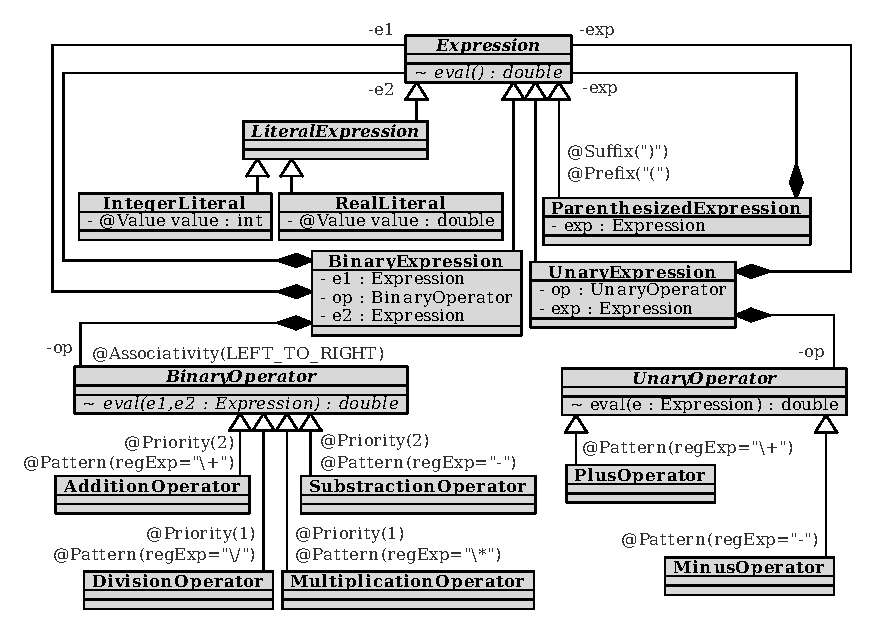
\includegraphics[width=1.00\textwidth]{calculator2.eps}\\[-1.5cm]

\subsubsection{Java class implementation}
The full functional implementation of this example (including valid import and package statements) can be found in the ModelCCExamples library, which is included in the source and binary distribution packages in the download section of the site (www.modelcc.org).

\begin{colframe}
\begin{verbatim}
public abstract class Expression implements IModel {
  public abstract double eval();
}

@Prefix("\\(") @Suffix("\\)")
public class ParenthesizedExpression
         extends Expression implements IModel {
  Expression e;
  @Override public double eval() {
    return e.eval();
  }
}

public abstract class LiteralExpression
         extends Expression implements IModel {
}

public class UnaryExpression
         extends Expression implements IModel {
  UnaryOperator op;
  Expression e;
  @Override public double eval() {
    return op.eval(e);
  }
}

public class BinaryExpression
         extends Expression implements IModel {
  Expression e1;
  BinaryOperator op;
  Expression e2;
  @Override public double eval() {
    return op.eval(e1,e2);
  }
}

public class IntegerLiteral
         extends LiteralExpression implements IModel {
  @Value int value;
  @Override public double eval() {
    return (double)value;
  }
}
\end{verbatim}
\end{colframe}

\begin{colframe}
\begin{verbatim}
public class RealLiteral
         extends LiteralExpression implements IModel {
  @Value double value;
  @Override public double eval() {
    return value;
  }
}

public abstract class UnaryOperator
         implements IModel {
  public abstract double eval(Expression e);
}

@Pattern(regExp="\\+")
public class PlusOperator
         extends UnaryOperator implements IModel {
  @Override public double eval(Expression e) {
    return e.eval();
  }
}

@Pattern(regExp="-")
public class MinusOperator
         extends UnaryOperator implements IModel {
  @Override public double eval(Expression e) {
    return -e.eval();
  }
}

@Associativity(AssociativityType.LEFT_TO_RIGHT)
public abstract class BinaryOperator
         implements IModel {
  public abstract double eval(Expression e1,Expression e2);
}

@Priority(value=2) @Pattern(regExp="\\+")
public class AdditionOperator
         extends BinaryOperator implements IModel {
  @Override public double eval(Expression e1,Expression e2) {
    return e1.eval()+e2.eval();
  }
}
\end{verbatim}
\end{colframe}

\begin{colframe}
\begin{verbatim}
@Priority(value=2) @Pattern(regExp="-")
public class SubstractionOperator
         extends BinaryOperator implements IModel {
  @Override public double eval(Expression e1,Expression e2) {
    return e1.eval()-e2.eval();
  }
}

@Priority(value=1) @Pattern(regExp="\\*")
public class MultiplicationOperator
         extends BinaryOperator implements IModel {
  @Override public double eval(Expression e1,Expression e2) {
    return e1.eval()*e2.eval();
  }
}

@Priority(value=1) @Pattern(regExp="\\/")
public class DivisionOperator
         extends BinaryOperator implements IModel {
  @Override public double eval(Expression e1,Expression e2) {
    return e1.eval()/e2.eval();
  }
}
\end{verbatim}
\end{colframe}

\subsection{Canvas Draw language} \label{sec:langcanv}

The Canvas Draw language allows the imperative generation of drawings.

\subsubsection{Language Specification}

The Canvas Draw language features the following capabilities:

\begin{itemize}
\item Setting the canvas width, height, and background color.
\item Changing the current color.
\item Changing the current stroke width.
\item Drawing lines, rectangles, circles, ovals, polygons, filled rectangles, filled circles, filled ovals, and filled polygons.
\item Each of the elements is described in a particular way (list of coordinates, coordinates and radius, ...).
\end{itemize}

Example input and output:
\begin{itemize}
\item Input:
\begin{verbatim}
   canvas                                 % Creates a canvas
        width 640                         % with width 640,
        height 480                        % height 480,
        background (92,164,169)           % and a cyan background.
                                          % Then:
      color (31,41,56)                    % Sets the color to dark cyan
      stroke 5                            % Sets the stroke to 5
      line [(10,10),(40,40)]              % Draws a line at (10,10) to (40,40)
      rectangle [(40,100),(60,120)]       % Draws a rectangle at (40,100) to (60,120)
      circle (400,30),400      
\end{verbatim}
\begin{itemize} \item Output: \\
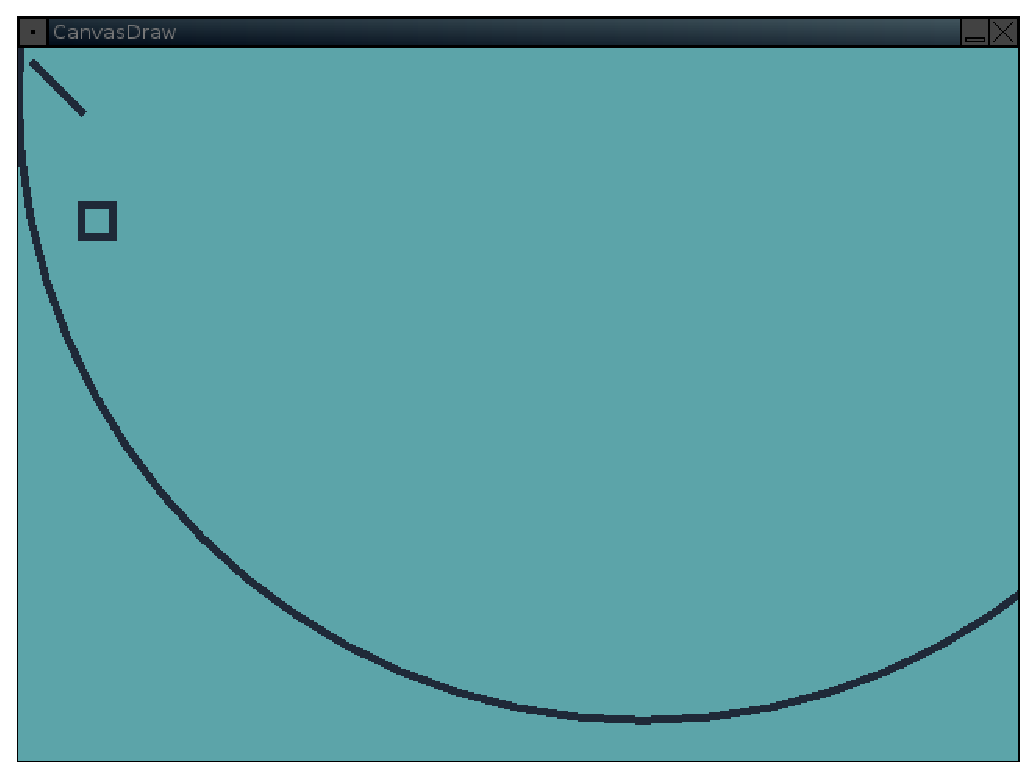
\includegraphics[width=0.70\textwidth]{canvas1.eps}
\end{itemize}

\item Input:
\begin{verbatim}
   canvas                                 % Creates a canvas
        width 800                         % with width 800,
        height 600                        % height 600,
        background (0,0,0)                % and a black background.
                                          % Then:
      color (180,40,40)                   % Sets the color to red
      rectangle [(40,100),(60,120)] fill  % Draws a fill rectangle at (40,100) to (60,120)
      oval [(300,200),(400,370)] fill     % Draws an oval at (300,200) to (400,370)
      stroke 3                            % Sets the stroke to 3
      line [(150,150),(200,200)]          % Draws a line at (150,150) to (200,200)
      color (40,180,40)                   % Sets the color to green
      stroke 7                            % Sets the stroke to 7
      circle (400,30),400                 % Draws a circle of radius 400 at (400,30)
      color (70,70,180)                   % Sets the color the purple
      polygon [(120,160),(110,140),       % Draws a fill polygon.
              (165,130),(186,180)] fill
\end{verbatim}
\begin{itemize} \item Output: \\
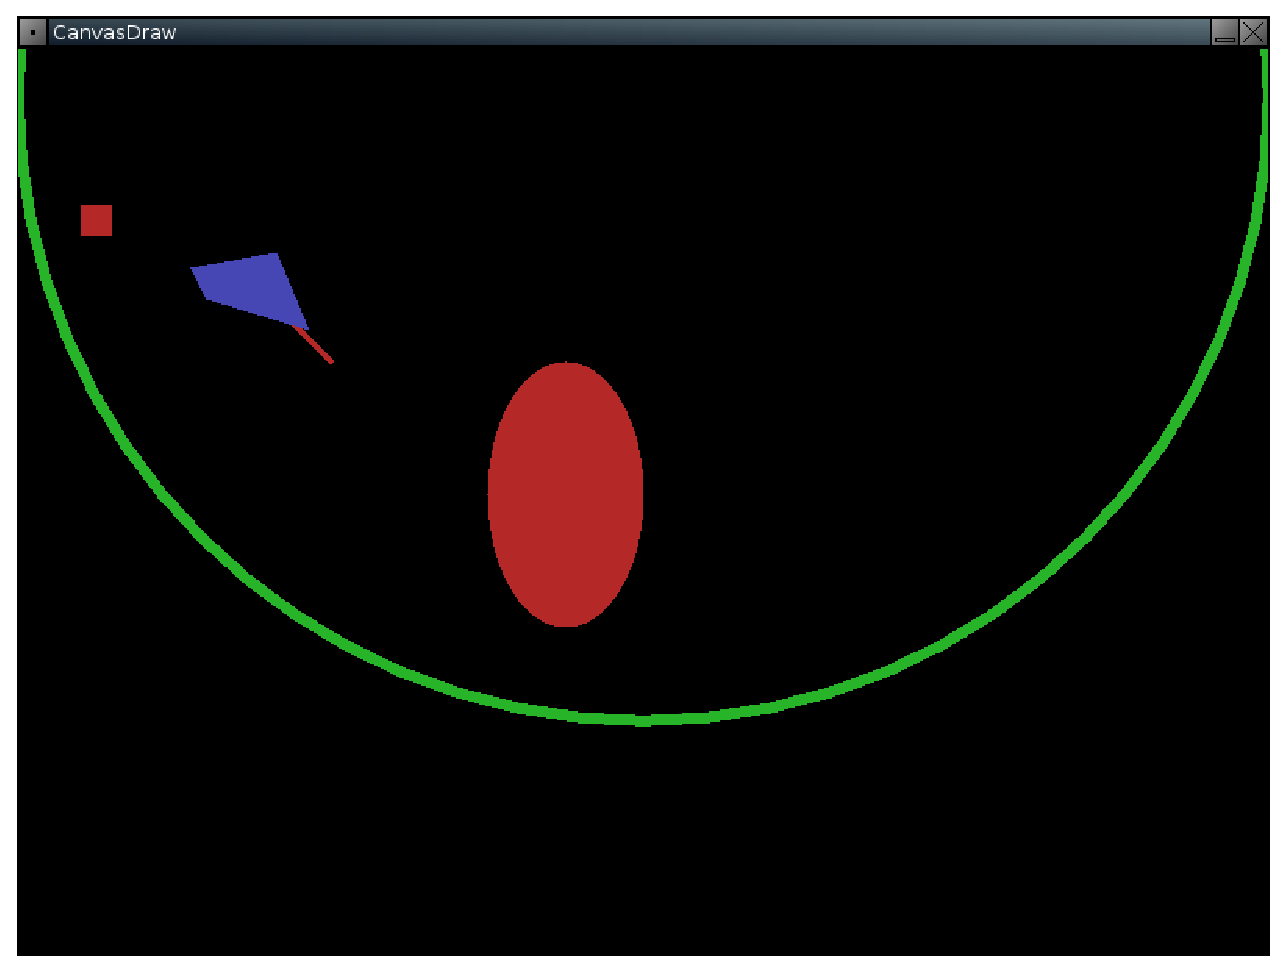
\includegraphics[width=0.80\textwidth]{canvas2.eps}
\end{itemize}
\end{itemize}


\subsection{Imperative Arithmetic language} \label{sec:langimpa}

The Imperative Arithmetic language processes processes assignment and output sentences containing arithmetic expressions in infix notation.

\subsubsection{Language Specification}
The Imperative Arithmetic language features the following capabilities:

\begin{itemize}
\item Unary operators: +, and -.
\item Binary operators: +, -, *, and /, being - and / left-associative.
\item Operator priorities: * and / precede + and -.
\item Parenthesized expressions.
\item Integer and floating-point literals.
\item Binary operators: +, and -.
\item Variables: different references to the same variable are links to the same object.
\end{itemize}

Example input and output:

\begin{itemize}
\item Input:
\begin{verbatim}
variables
  var a
  var b
  var c
sentences
  a = 1
  b = a+2
  c = (a+b)*2
  output a
  output b
  output c
\end{verbatim}
\begin{itemize} \item Output:
\begin{verbatim}
1.0
3.0
8.0
\end{verbatim}
\end{itemize}
\end{itemize}

\section{Testing} \label{sec:testing}

This section presents an example on model testing using the ModelCC testing framework.

ModelCC's ModelAssert class provides static assert methods that allow embedding unitary model tests in code.

\begin{colframe}
\begin{verbatim}
import static org.modelcc.test.ModelAssert.*;

try {

    Model model = JavaModelReader.read(Expression.class);
    Set<PatternRecognizer> se = new HashSet<PatternRecognizer>();
    se.add(new RegExpPatternRecognizer(" "));
    Parser<Expression> parser = ParserFactory.create(model,se);

    assertValid(parser,"1+2");
    assertValid(parser,"1+ 2");
    assertInvalid(parser,"a1+2");
    assertAmbiguityFree(parser,"1+2");
    assertInterpretations(1,parser,"1+2+5");

} catch (Exception ex) {
    assertFalse(true);
    return;
}
\end{verbatim}
\end{colframe}

%\fancyhead[LE]{}
%\newpage
%\bibliographystyle{abbrv}
%\bibliography{doc}
%\fancyhead[LE]{\rightmark}

%\newpage
%\pagestyle{empty}
%\cleardoublepage
%\empt
%\rule{0cm}{10cm}
%\begin{center}
%ModelCC User Guide
%\end{center}
\end{document}



